 \documentclass{article}
\usepackage{setspace,tikz,wrapfig}
\usepackage[text={6.5in,8.5in},centering]{geometry}
\geometry{verbose,a4paper,tmargin=2.4cm,bmargin=2.4cm,lmargin=2.4cm,rmargin=2.4cm}
\usepackage{graphicx,amsmath,cases,multirow,appendix,graphicx,xcolor}
\usepackage[makeroom]{cancel}

\setlength\parindent{0pt}

\newcommand{\note}[1]{\colorbox{gray!30}{#1}}
\newcommand{\ind}{\-\hspace{1cm}}
\newcommand*\circled[1]{\tikz[baseline=(char.base)]{
            \node[shape=circle,draw,inner sep=2pt] (char) {#1};}}
\newenvironment{rcases}
  {\left.\begin{aligned}}
  {\end{aligned}\right\rbrace} 
  
  
\renewcommand\floatpagefraction{.9}
\renewcommand\topfraction{.9}
\renewcommand\bottomfraction{.9}           


\begin{document}

\noindent\makebox[\textwidth][c]{\Large\bfseries Lecture 17 -- Tipping Points}

\textbf{Concepts:}\\
\ind - Alternative Stable States\\
\ind - Hysteresis\\
\ind - System potential\\
\ind - Critical slowing down and early-warning signals

\rule[0.5ex]{\linewidth}{1pt}
\textbf{Alternative Stable States}\\
 $\Rightarrow$ `Two (or more) equilibria under \emph{the same} conditions'\\
e.g., LV competition model\\
\ind Saddle-node bifurcation when \emph{inter-} $>$ \emph{intra}-specific competition\\
\ind \ind Either 1st of 2nd species persists, depending on initial conditions (\emph{Priority effect})\\

Contrast to \emph{Phase shift}\\
 $\Rightarrow$ `Different community structure under \emph{different} conditions'\\
 
Today -- \emph{Fold bifurcation}:  Alternative Stable States due to combination of:\\
\ind 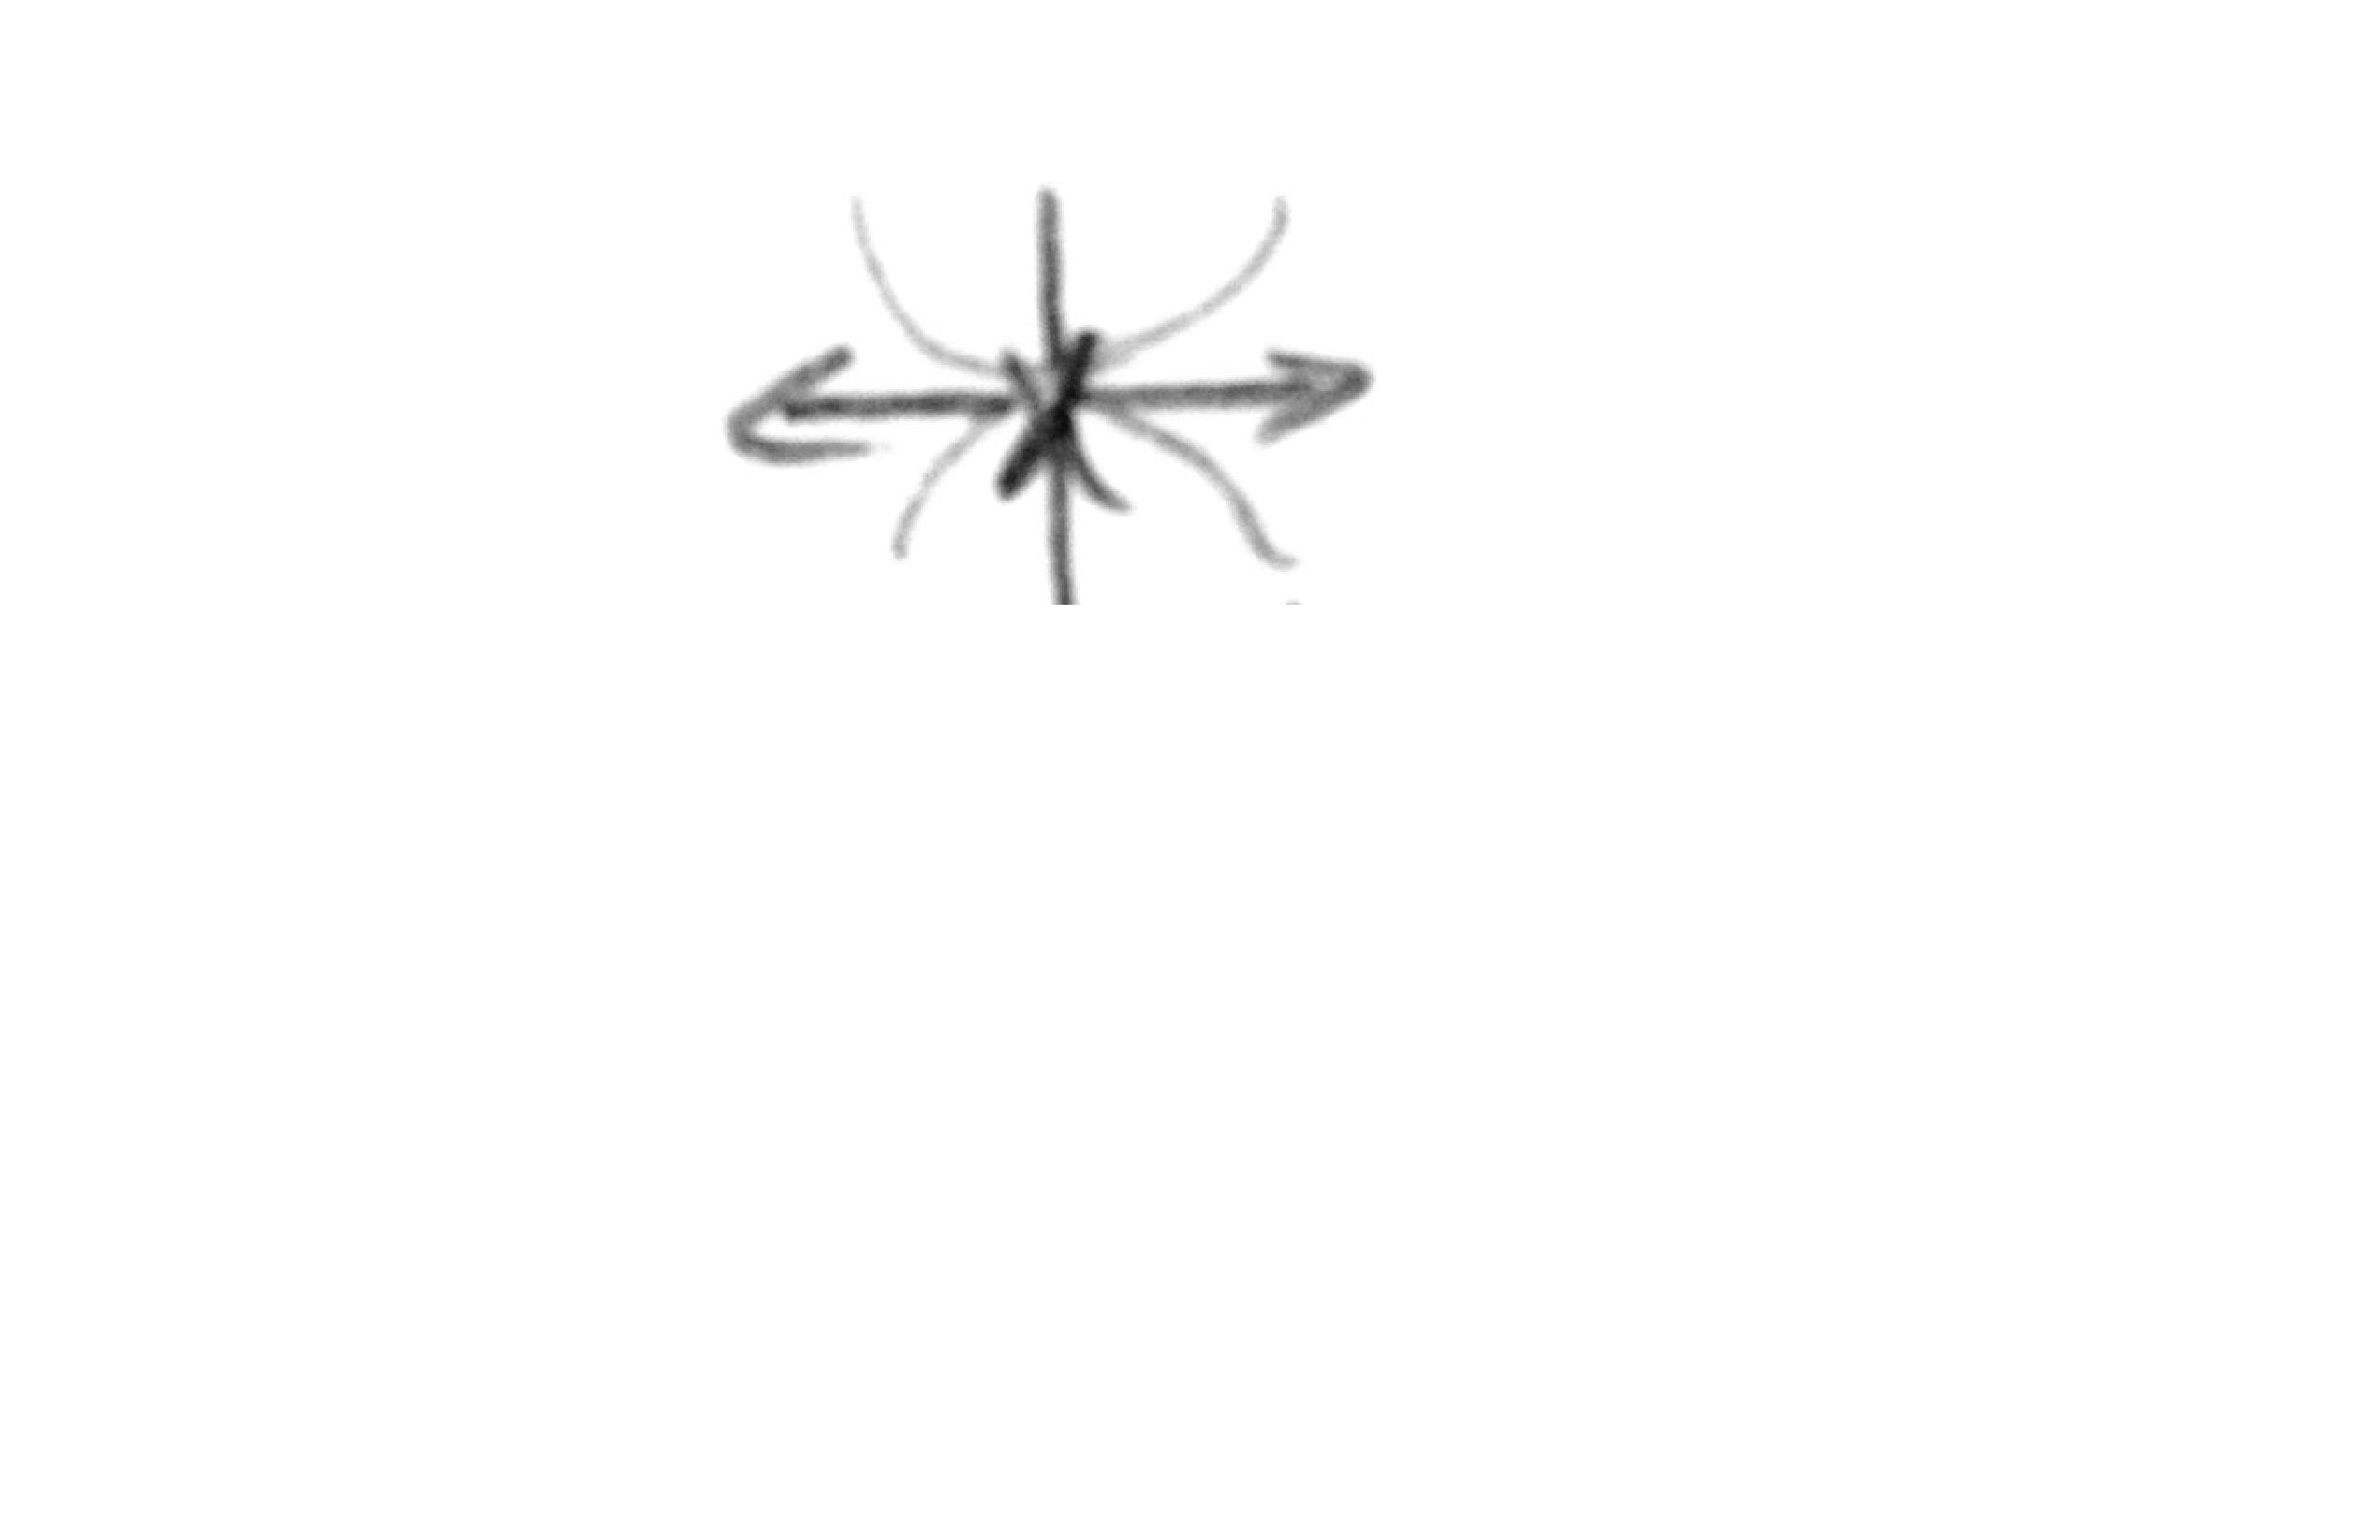
\includegraphics[width=2cm]{figs/SaddleNode.pdf} \ind  \emph{Saddle-node bifurcation}\\
\ind and\\
\ind  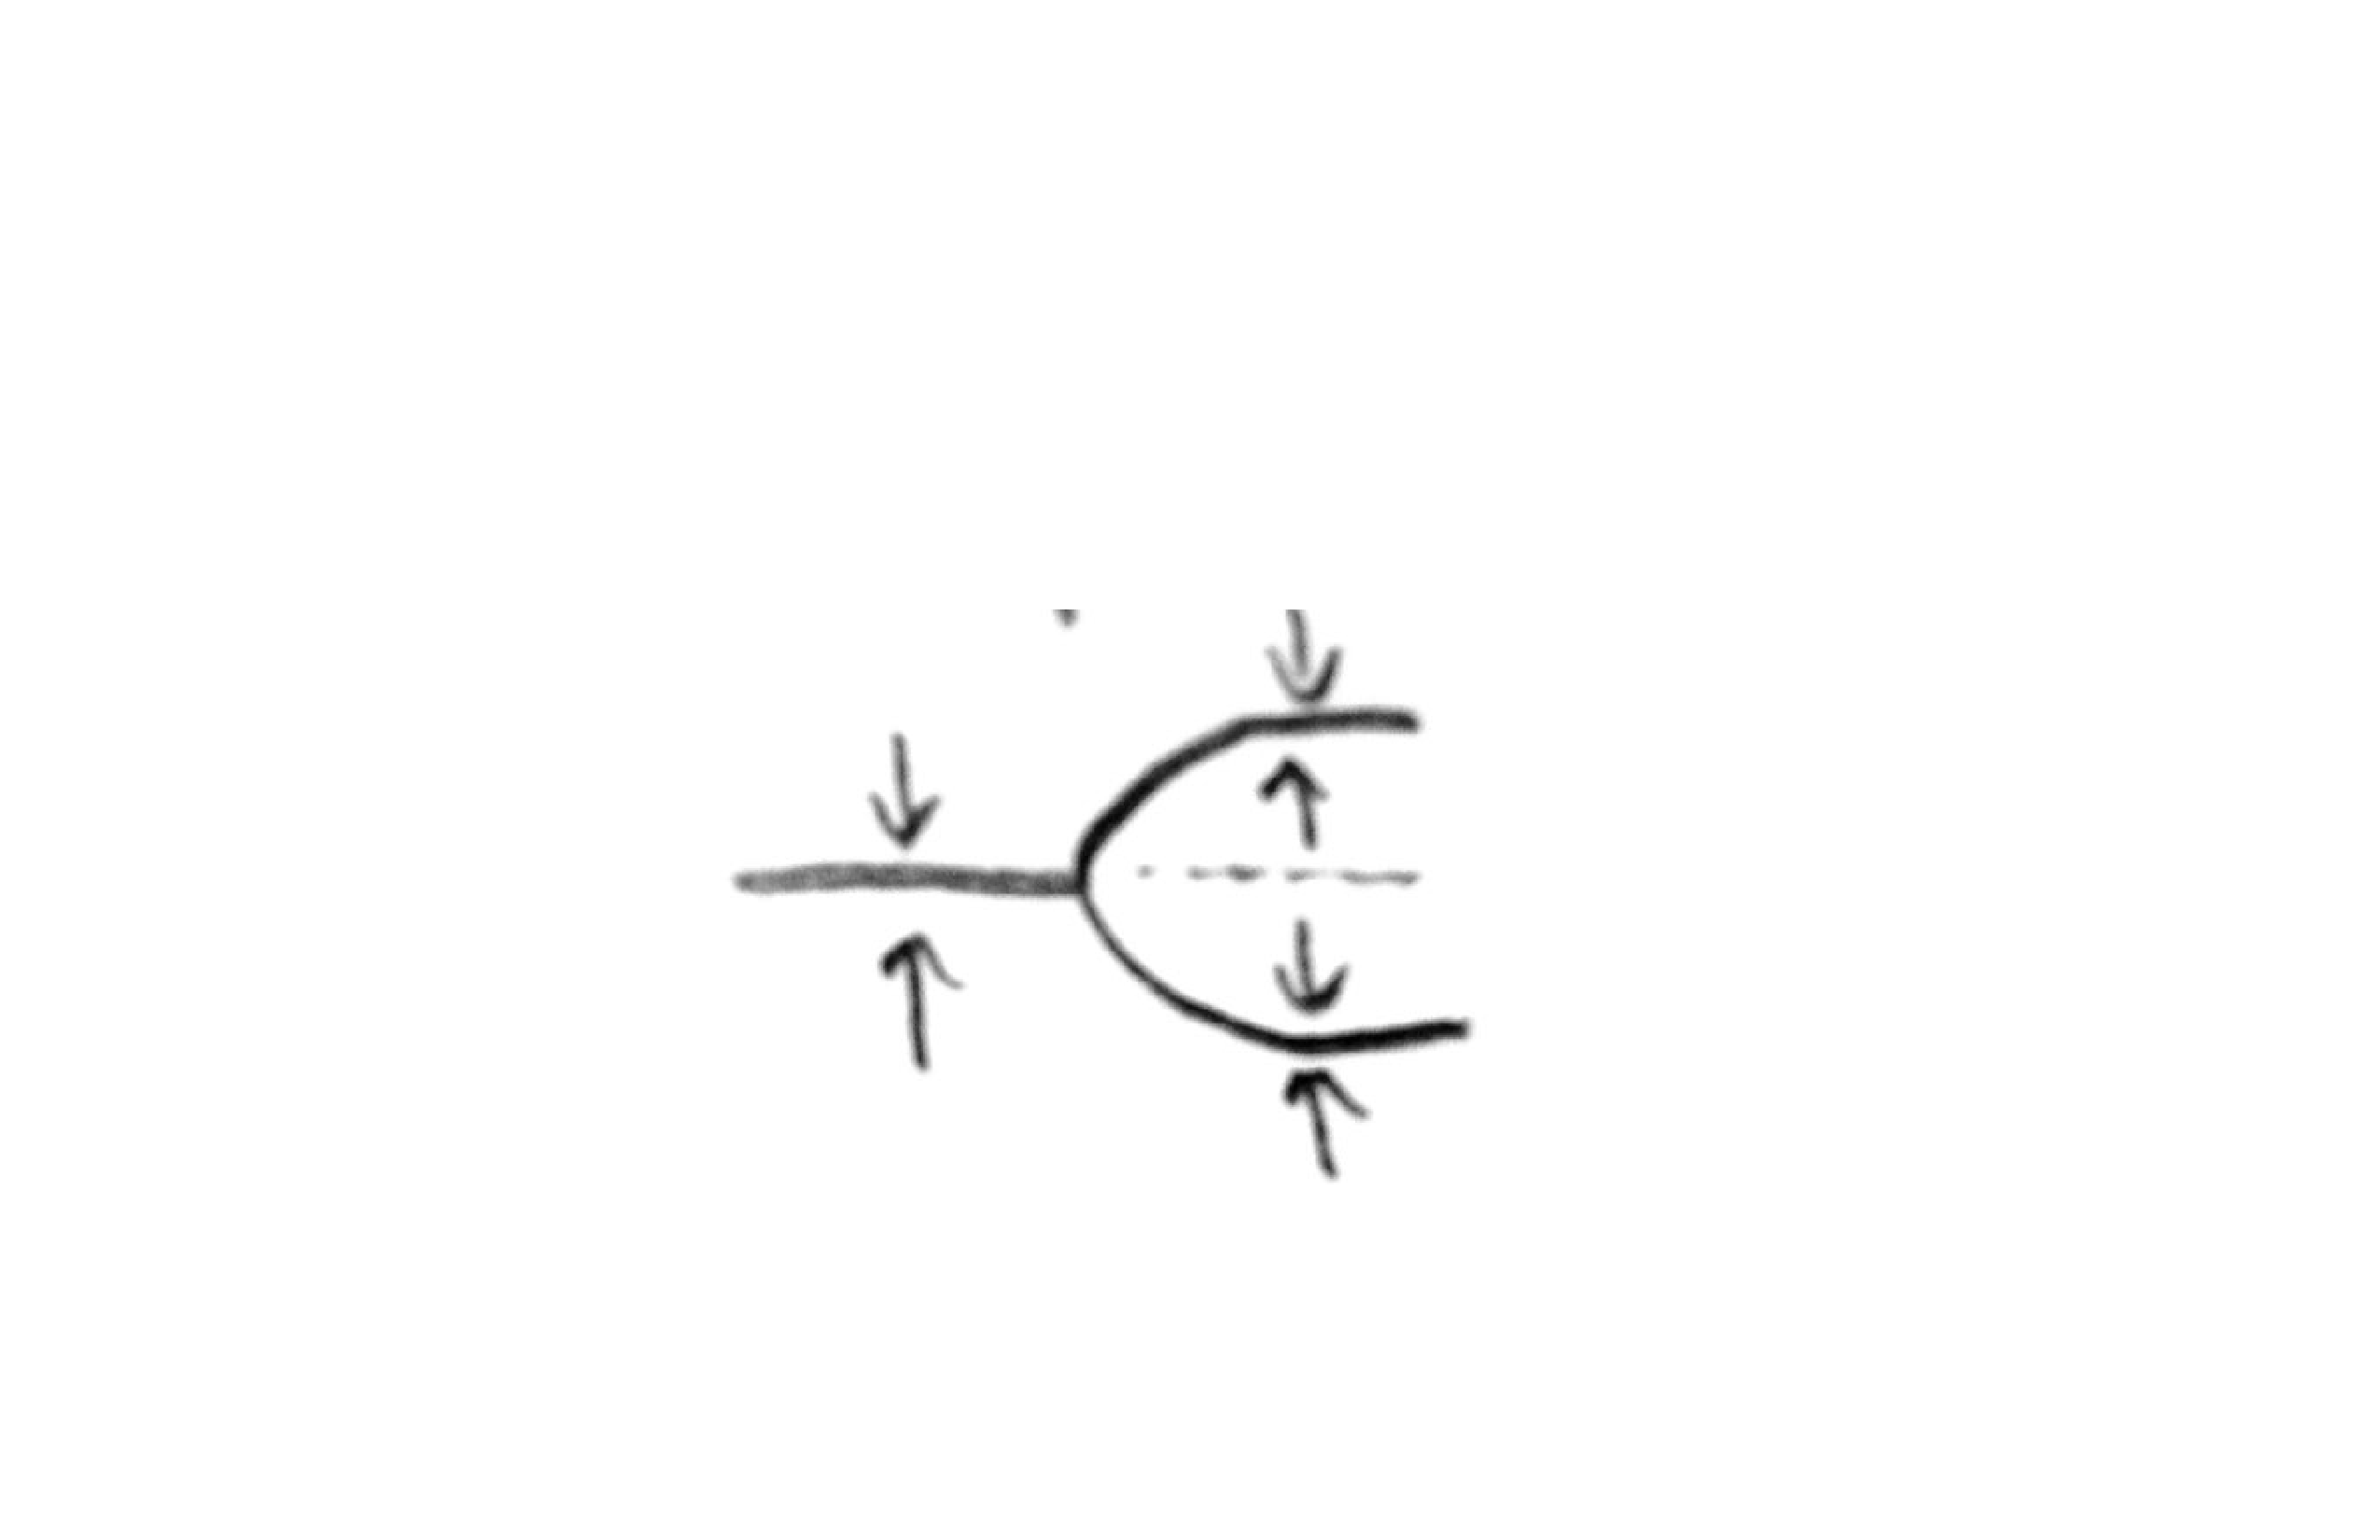
\includegraphics[width=2cm]{figs/Pitchfork.pdf}\ind \emph{Pitchfork bifurcation}\\

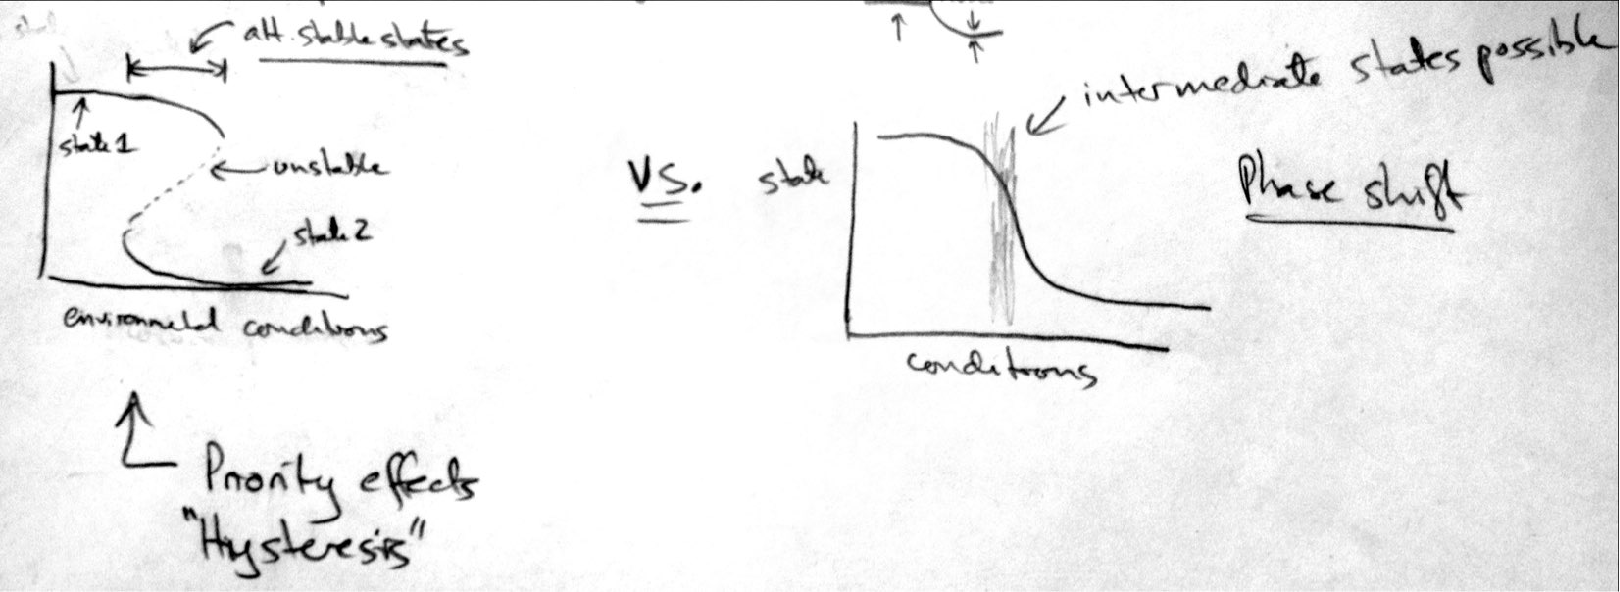
\includegraphics[width=16cm]{figs/Fold_vs_Phase.pdf}


\rule[0.5ex]{\linewidth}{1pt}
\textbf{System Potential}\\
Ball \& cup diagram is not just an analogy!\\

Example: Logistic w/ Allee Effect\\
\begin{equation*}
	\frac{dN}{dt}=rN\left(1-\frac{N}{K}\right)\left(\frac{N}{A}-1\right)
\end{equation*}
\ind (Note slightly different formulation that in Problem Set, but same effect.)
\begin{center}
 	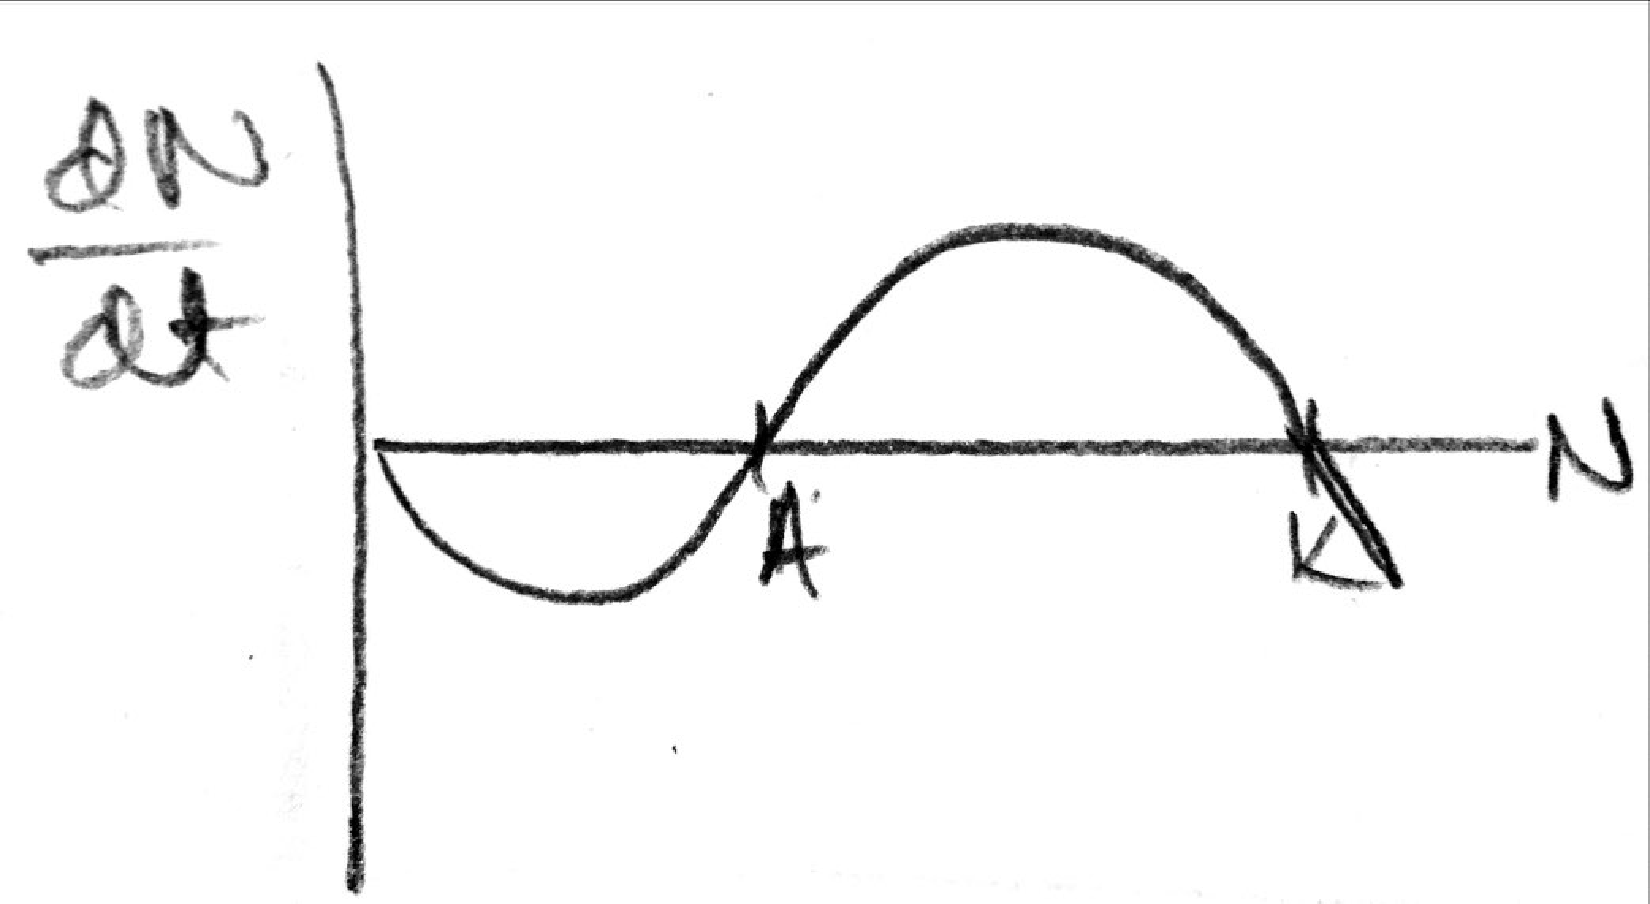
\includegraphics[width=5cm]{figs/LogisticAllee.pdf}
\end{center}
\pagebreak
\textbf{1.} Solve for equilibria. \ind \textbf{2.} Determine stability. \ind \textbf{3.} Interpret.\\
\note{$\Rightarrow$ Mathematica}
\begin{align*}
N^*=\begin{cases}
	0\\
	A\\
	K
\end{cases}\qquad
\frac{d\tfrac{dN}{dt}}{dN}=\begin{cases}
	-r\\
	r-\frac{A}{K}r>0 \text{ when }A<K \\
	r-\frac{K}{A}r<0 \text{ when }A>K 
\end{cases}\qquad
\Rightarrow\begin{cases}
	\text{ stable}\\
	\text{ unstable}\\
	\text{ stable}
\end{cases}
\end{align*}
Therefore
\begin{align*}
	N_0<A &\Rightarrow N_t \to 0\\
	N_0>A &\Rightarrow N_t \to K
\end{align*}
Def. System Potential (\emph{Phi}):
\begin{equation*}
	\boxed{\Phi=-\int_{-\infty}^{\infty}\frac{dN}{dt} dN}
\end{equation*}
$\int \frac{dN}{dt} dN$ is nothing more than area under the curve in plot of $\frac{dN}{dt}$ vs. $N$
\begin{center}
 	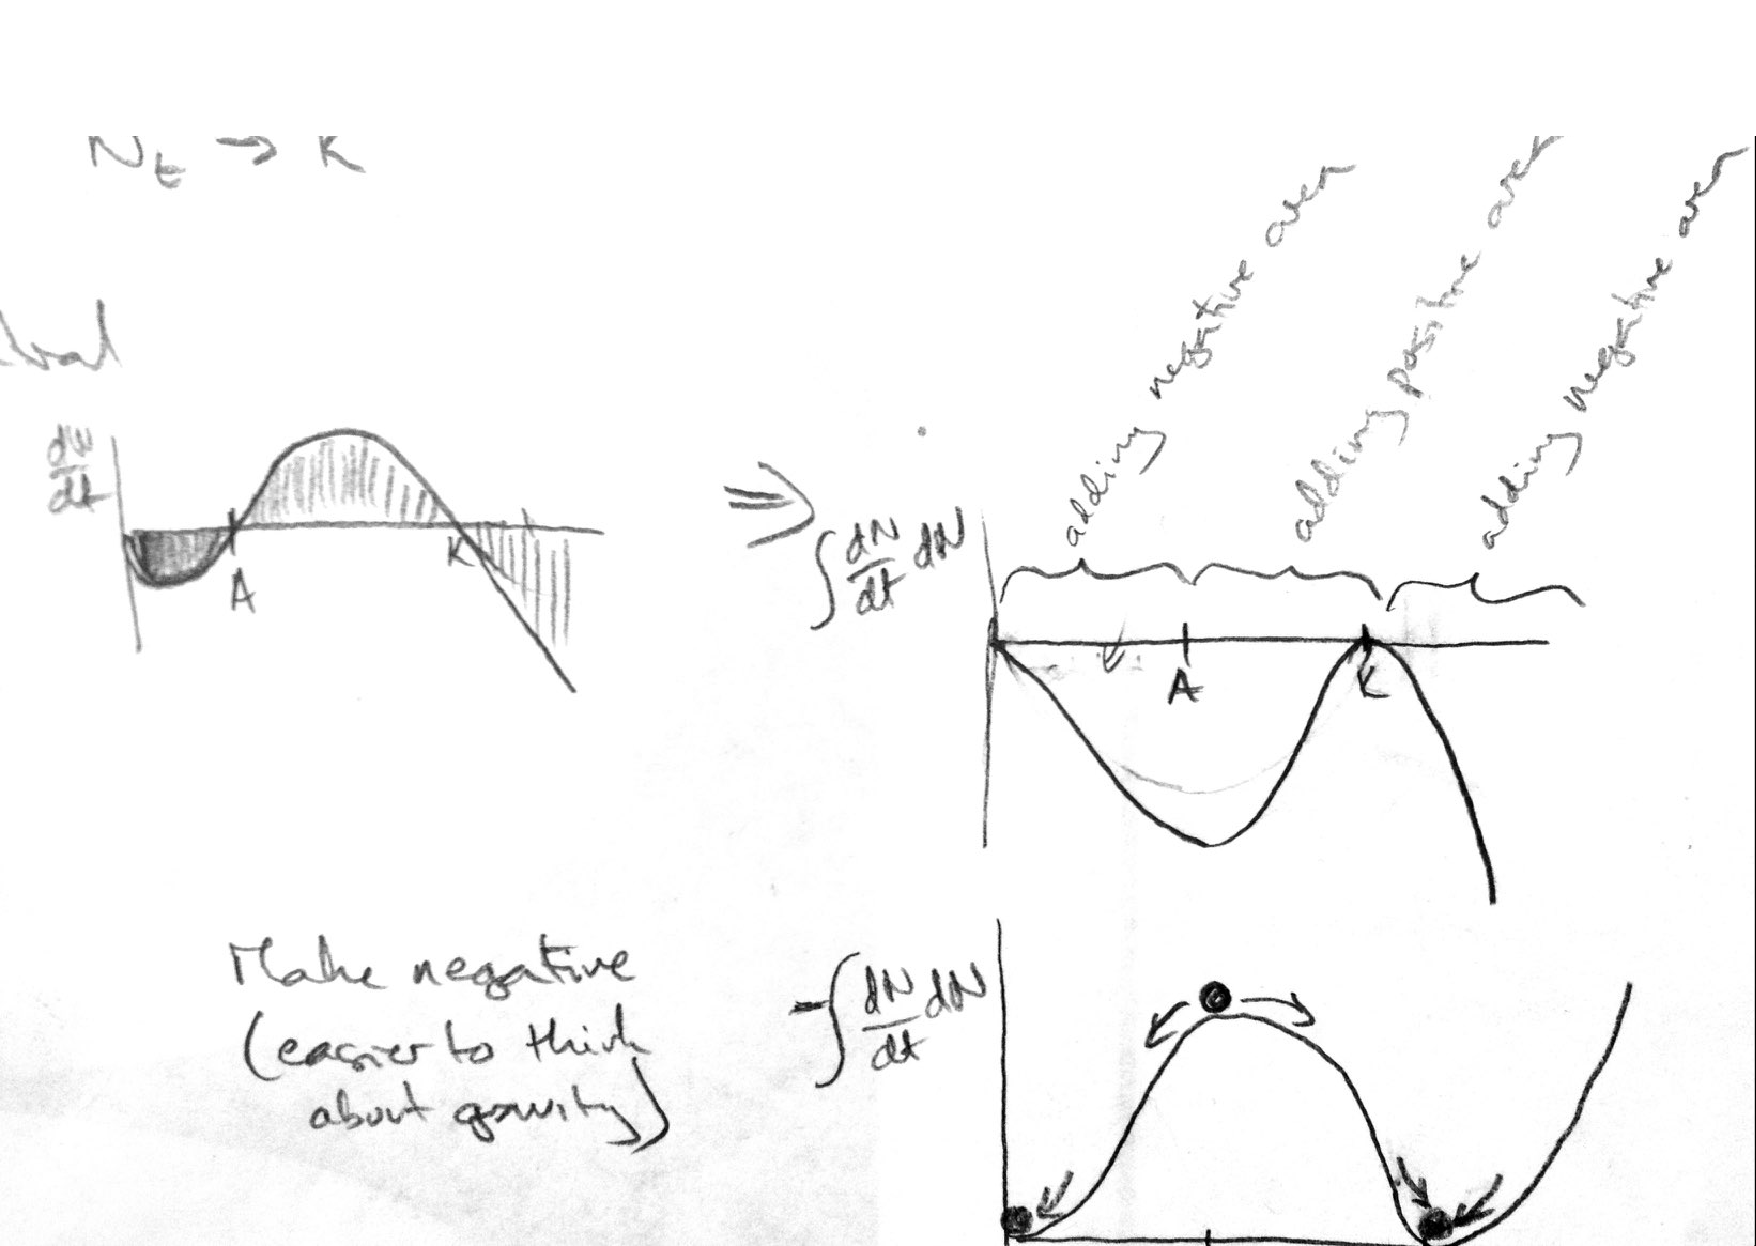
\includegraphics[width=14cm]{figs/LogisticAllee_Potential.pdf}
\end{center}

\rule[0.5ex]{\linewidth}{1pt}
\textbf{Exploitation model}\\
\ind (commonly used model to illustrate tipping points)
\begin{equation*}
	\frac{dN}{dt}=rN\left(1-\frac{N}{K}\right) - \frac{cN^2 P}{b+N^2}
\end{equation*}
\ind = Logistic growth with Type 3 functional response.

\rule[0.5ex]{5cm}{1pt}

\emph{Side-note on functional response formulation:}\\
Holling Type II:
\begin{align*}
	f(N)=\frac{aN}{1+ahN} \qquad \qquad a \text{ - per capita attack rate } \qquad h \text{ - handling time}
\end{align*}
\begin{center}
 	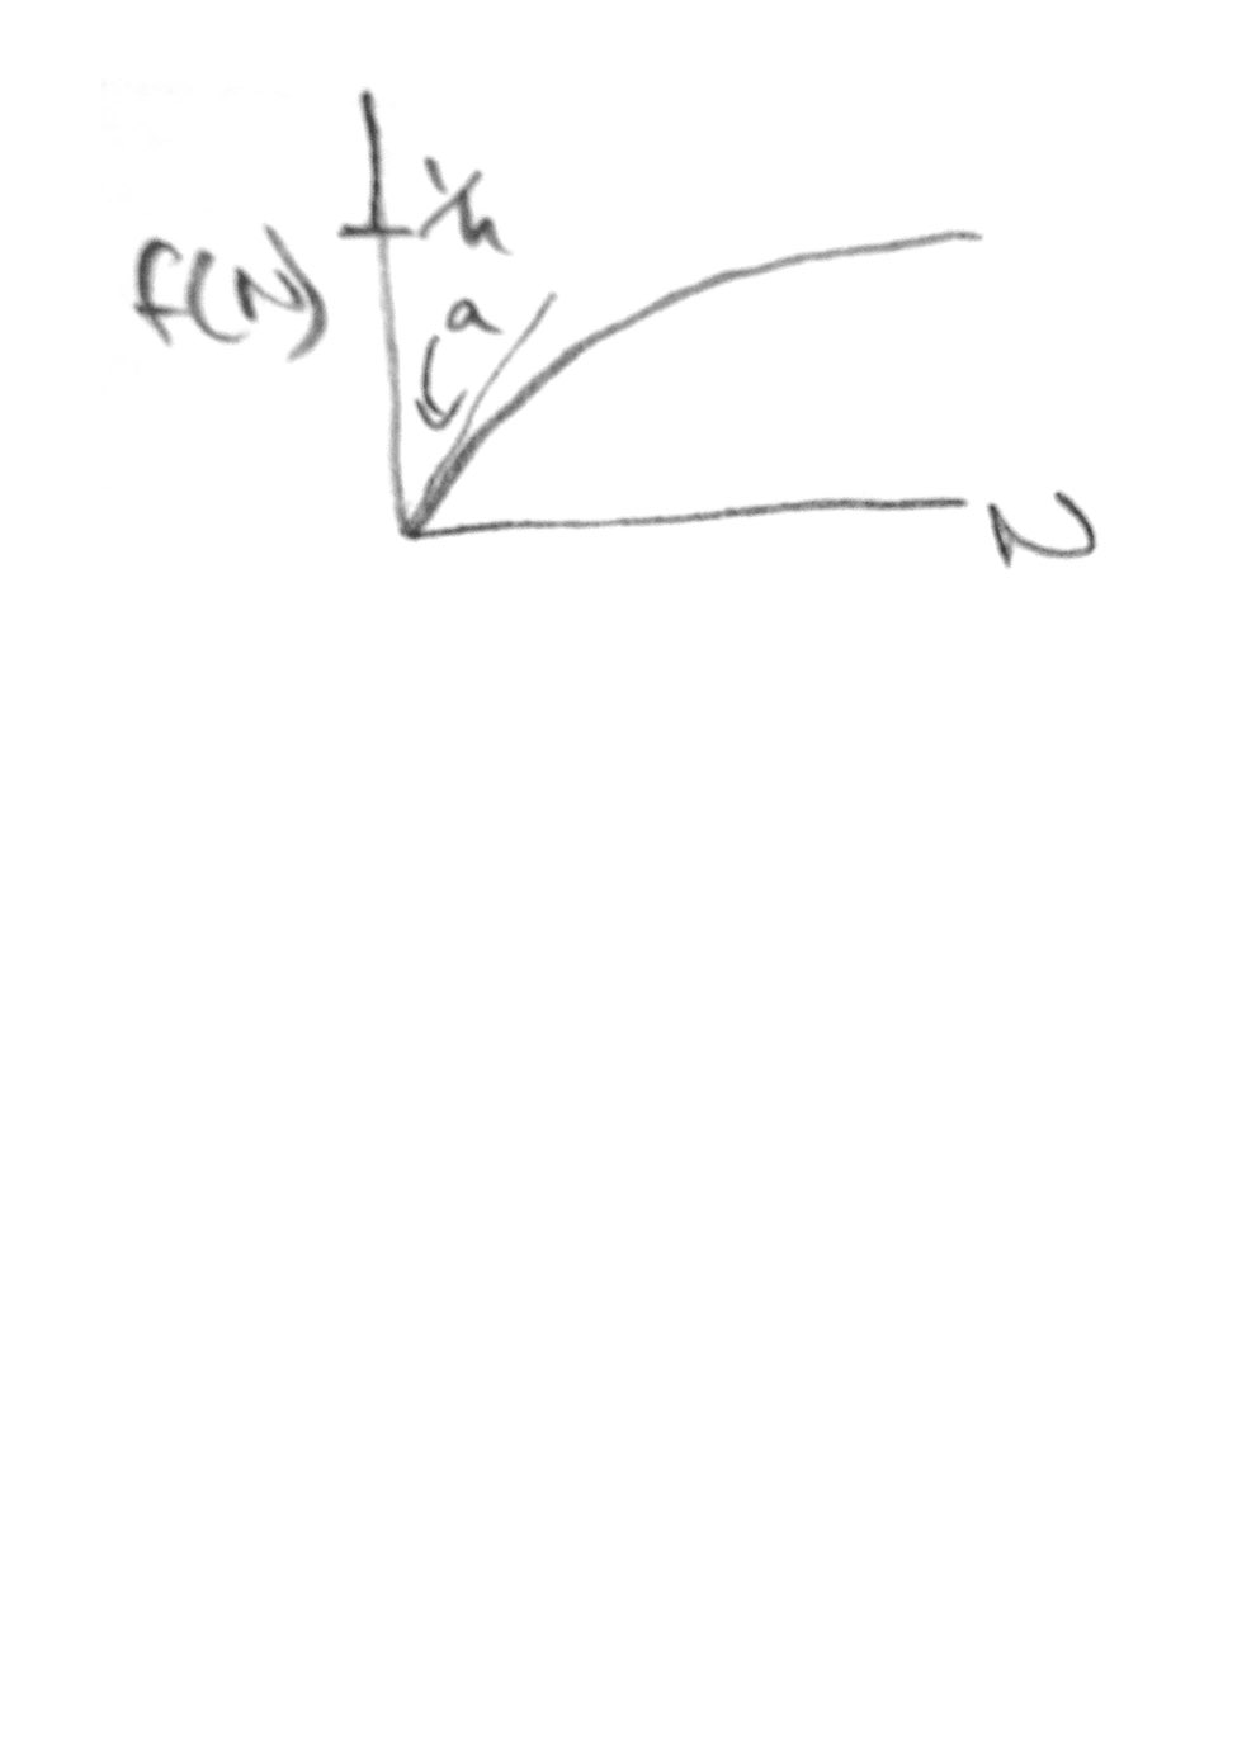
\includegraphics[width=3cm]{figs/TypeII-Holling.pdf}
\end{center}
 Michaelis-Menten:
\begin{equation*}
	f(N)=\frac{cN}{b+N} \qquad \qquad c \text{ - maximum feeding rate (capacity)}= \frac{1}{h} \qquad b \text{ - half-saturation constant} = \frac{1}{ah}
\end{equation*}
\begin{center}
 	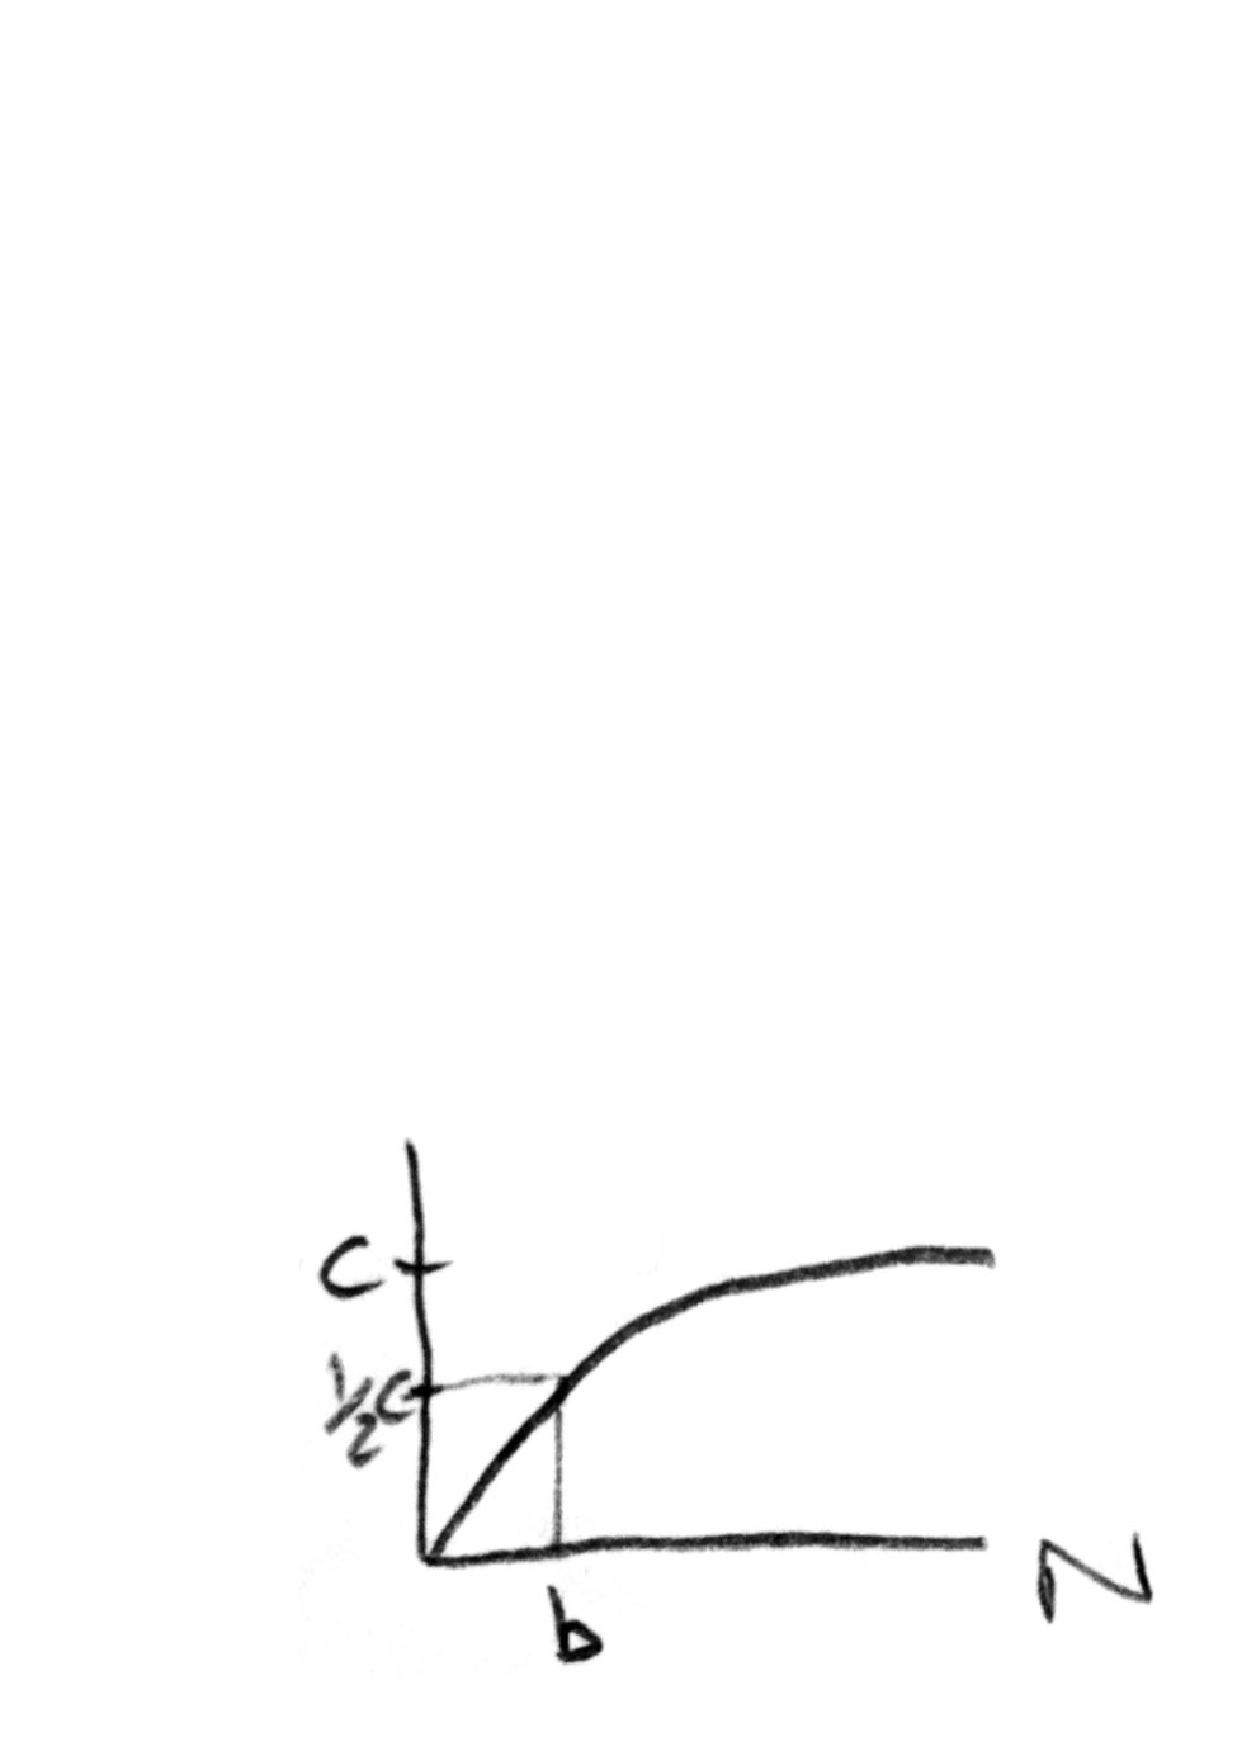
\includegraphics[width=2.5cm]{figs/TypeII-MM.pdf}
\end{center}

Holling Type III:
\begin{equation*}
	f(N)=\frac{aN^m}{1+ahN^m} \Rightarrow  \frac{cN^2}{b+N^2}  \qquad \qquad m - \text{ Hill exponent, typically set to }m=2
\end{equation*}

\rule[0.5ex]{5cm}{1pt}

\textbf{Exploitation model}\\
\ind Let $P=1$ (fixed, arbitrary.  Limited by something else.)\\
\textbf{1.} Solve for equilibria: \note{$\Rightarrow$ Mathematica}
\begin{align*}
N^*=\begin{cases}
	0\\
	>0\\
	\text{crazy looking symbolically}\\
	\text{crazy looking symbolically}
\end{cases}
\end{align*}
\textbf{2.} Plot equilibria as function of control parameter $c$\\
\ind \ind ($c$ = feeding capacity, i.e.\emph{maximum exploitation rate})
\begin{center}
 	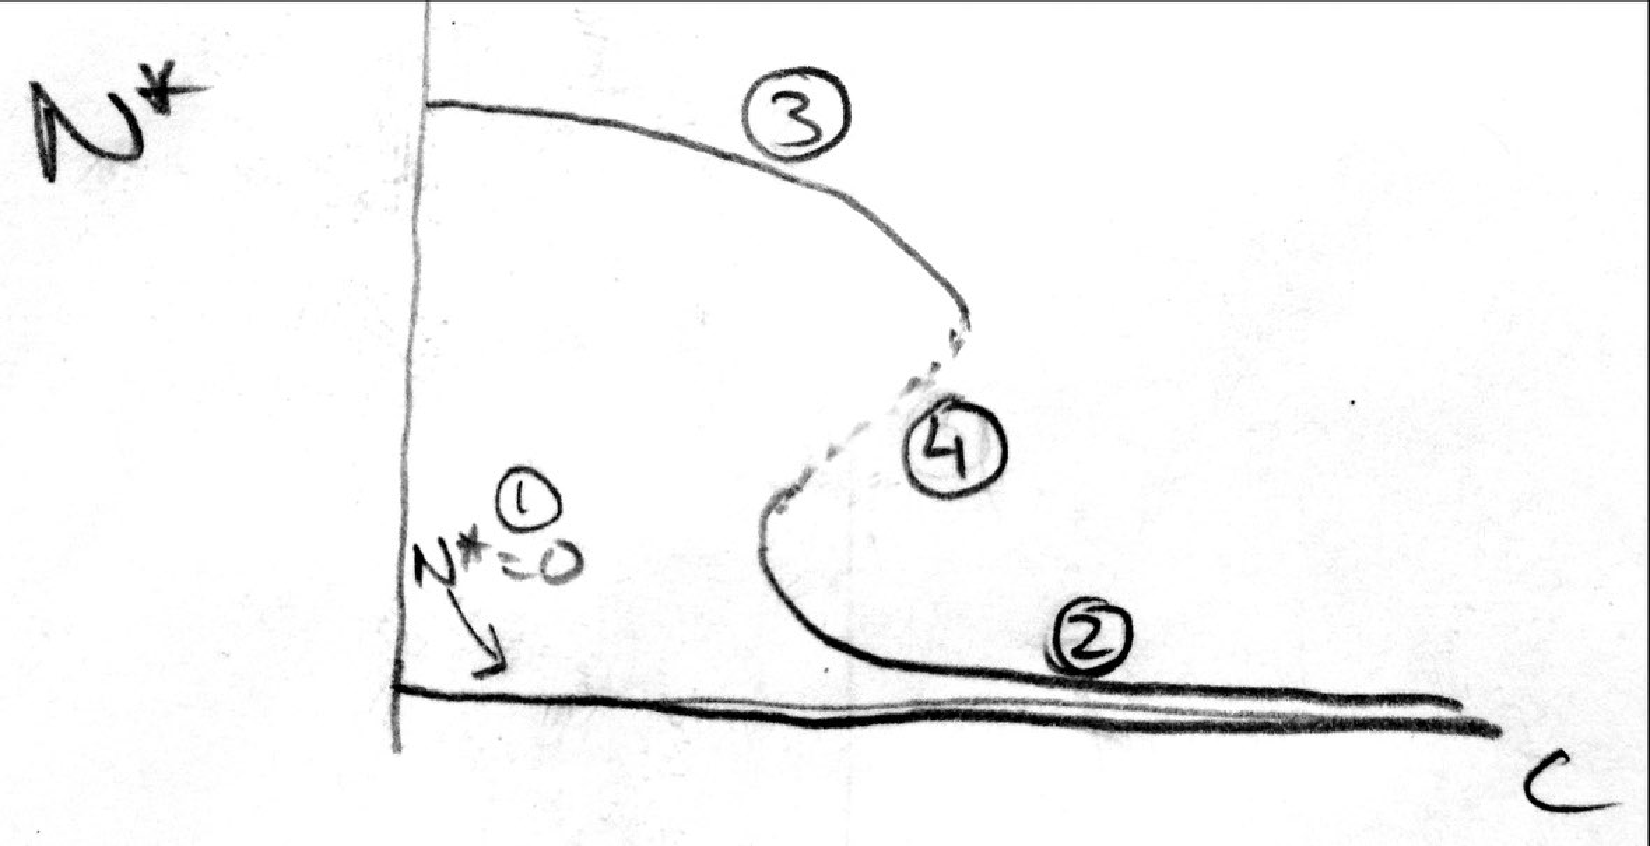
\includegraphics[width=6cm]{figs/Exploitation_Fold.pdf}
\end{center}
\textbf{3.} Determine stability\\
\begin{equation*}
	\frac{d\frac{dN}{dt}}{dN}=\lambda = \frac{2cN^3P}{(b+N^2)^2}-\frac{2cNP}{b+N^2}-\frac{rN}{K}+r\left(1-\frac{N}{K}\right)
\end{equation*}
\textbf{4.} Evaluate $\lambda$ at $N^*$ and plot as function of control parameter $c$
\begin{center}
 	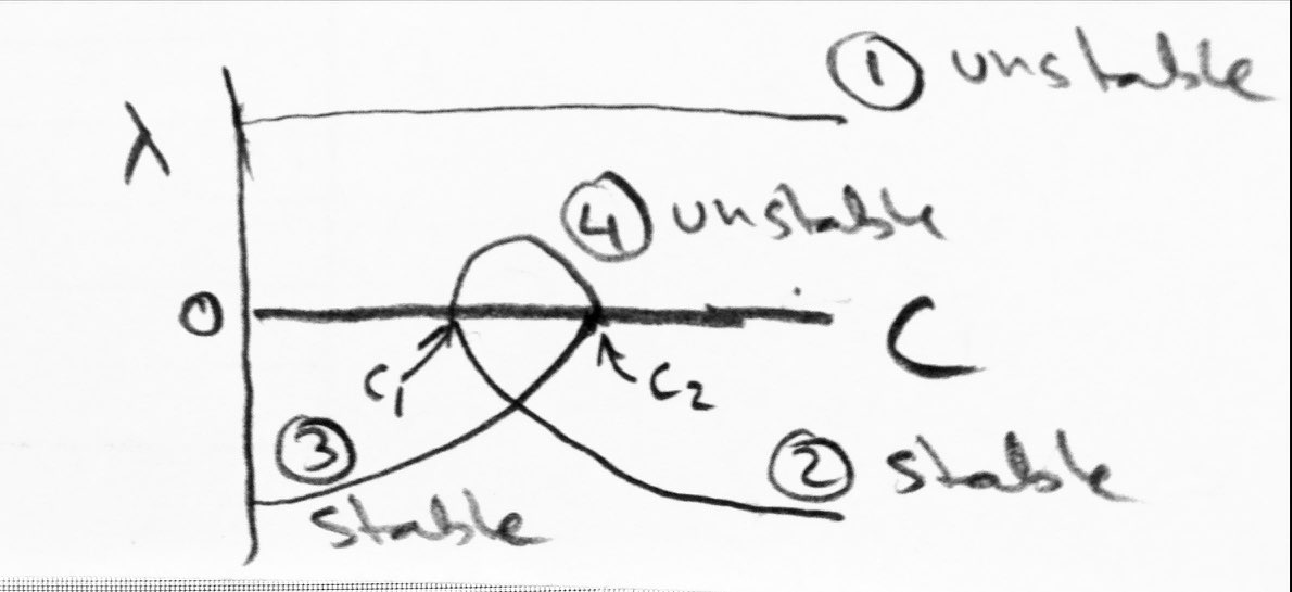
\includegraphics[width=6cm]{figs/Exploitation_Eigenvalue.pdf}
\end{center}
Unstable trivial equilibrium \circled{1}  $\Rightarrow$ Popn will always be present unless extinct.\\
Unstable non-trivial equilibrium \circled{4} sandwiched between two stable equilibria \circled{2} and \circled{3}\\

Starting in \circled{3}, increasing $c$ causes $\lambda \to 0$, then passing critical value $c_2$ causes $\lambda << 0$ jump.\\
Starting in \circled{2}, decreasing $c$ causes $\lambda \to 0$, then passing critical values $c_1$ causes $\lambda << 0$ jump.\\

$\Rightarrow$ Two \textbf{`Critical transitions'}\\
\ind Small changes in control parameter causes large `catastrophic' change in system state\\
To get back to `old' state requires larger reversal of control parameter than what caused shift.\\
\ind \textbf{\emph{Hysteresis}}\\

Fishery context - harvest rate\\
\ind Slow increase causes only small decrease in stock size until, all of a sudden, stock crashes.\\
\ind Pulling back a little makes little difference due to hysteresis.\\

\rule[0.5ex]{\linewidth}{1pt}

\textbf{System Potential \& Critical slowing down}\\
\begin{equation*}
\Phi=-\int \frac{dN}{dt}dN
\end{equation*}
\ind \note{$\Rightarrow$ Mathematica (First Manipulate plot of $c$)}\\
\begin{center}
 	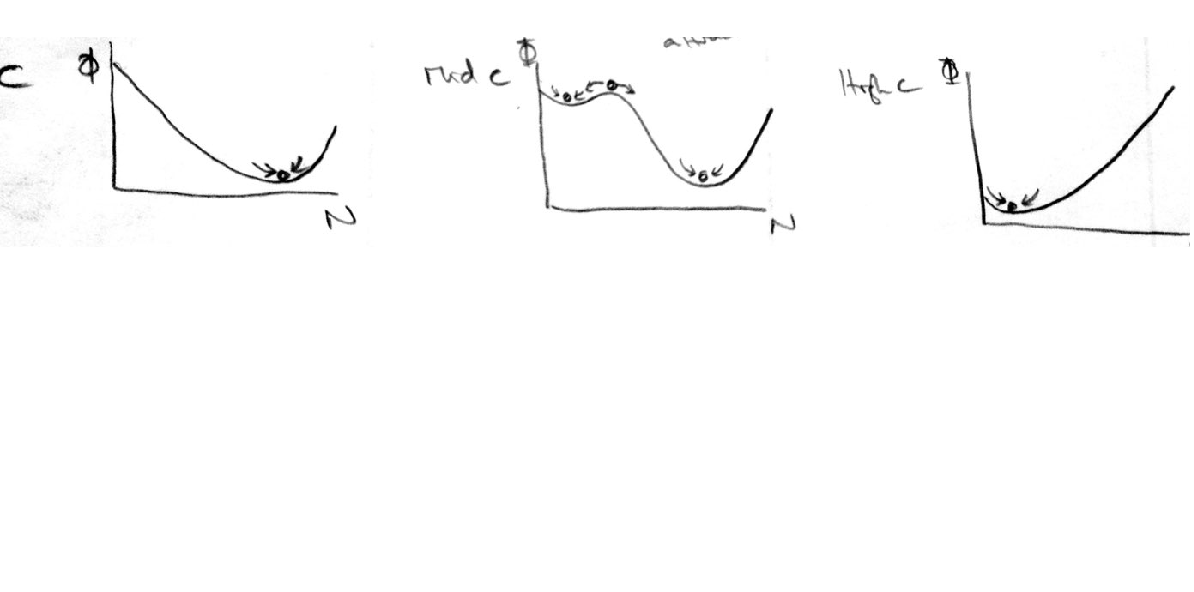
\includegraphics[width=15cm]{figs/Exploitation_SysPot.pdf}
\end{center}
Observe that the landscape flattens out near critical values $c_1$ and $c_2$ where the 2nd basin emerges.
\begin{center}
 	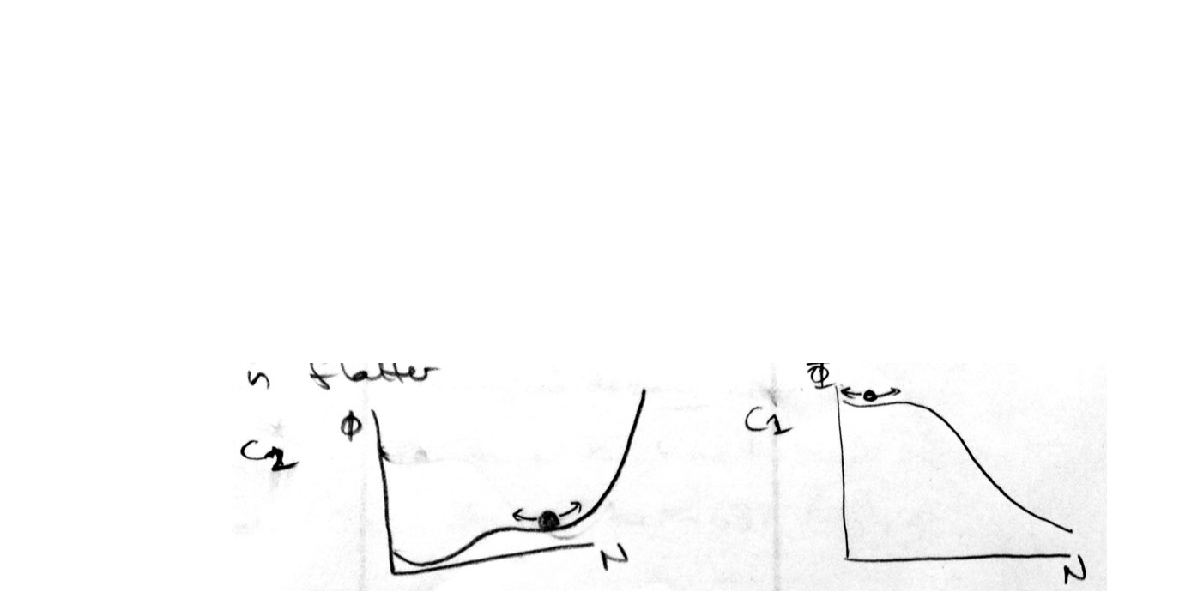
\includegraphics[width=10cm]{figs/Exploitation_SysPot_c.pdf}
\end{center}
\begin{equation*}
\text{As }\lambda \to 0 \; \;  \Rightarrow \;\; \underbrace{\frac{d (- \int \frac{dN}{dt}dN)}{dN}}_{\text{slope} =-\frac{dN}{dt}} \to 0
\end{equation*}
Thus intuitively:  If we perturb the system, it should respond slower.
\begin{center}
 	
\includegraphics[width=5cm]{figs/BallCup.pdf}
\end{center}
\pagebreak
Evaluate intuition formally:

\begin{minipage}[t]{0.3\textwidth}
	\begin{center}\textbf{1-sp.}\end{center}
	\circled{1} Solve for equil
	\begin{align*} \frac{dN}{dt}&=f(N)=0\\&\Rightarrow N^*\end{align*} \\
	\circled{2} Determine stability of $N^*$\\
	\ind Determine\\
		\begin{equation*} \frac{d f(N)}{dN} \end{equation*}
	\ind Evaluate at $N^*$\\
		\begin{equation*} \left.\frac{d f(N)}{dN}\right\vert_{N^*}=\lambda \end{equation*}\\ \\ \\ \\ \\ \\
	\circled{3} Interpret $\lambda$'s\\
	\ind $x = $ perturbation
	\begin{align*}	\frac{dx}{dt}&=\lambda x\\ \Rightarrow  x_t &=x_0 e^{\lambda t}	\end{align*}
	\ind Stable if $Re(\lambda) < 0 $
\end{minipage}
\begin{minipage}[t]{0.3\textwidth}
	\begin{center}\textbf{1-sp. example}\end{center}
	\begin{align*}\frac{dN}{dt}& =rN\left(1-\frac{N}{K}\right)=0\\\Rightarrow & N^*= \begin{cases} 0\\K \end{cases}\end{align*}\\ \\
	\begin{equation*}	r-2r\frac{N}{K}	\end{equation*}\\
	\begin{align*} r-2r \frac{K}{K}\\=r-2r\\=-r	\end{align*} \\ \\ \\ \\ \\ 
	\begin{align*}	\frac{dx}{dt}&=-rx\\ \Rightarrow x_t &= x_0 e^{-rt}
	\end{align*}
	\ind \ind $\Rightarrow$ Stable
\end{minipage}
\begin{minipage}[t]{0.3\textwidth}
	\begin{center}\textbf{n-spp.}\end{center}
	\begin{align*}\frac{dN_i}{dt}& =f_i(\vec{N})=0\; \forall i\\\Rightarrow & \vec{N}^*\end{align*}\\ \\ \\
	\ind Evaluate\\
	\begin{equation*} \mathbf{A}=\frac{\partial f_i(\vec{N})}{\partial N_j} \; \; \forall i,j	\end{equation*}\\ \\
	\begin{equation*} \mathbf{A}\vert_{N^*}	\end{equation*}
	 (i) Routh-Hurwitz Criteria\\
	 (ii) Eigenvalues $\lambda_i$ (\emph{scalar representation of Jacobian transformation matrix})\\ \\ \\ 
	 \begin{align*}
		 \vec{n}=\begin{bmatrix} x\\y\\z \end{bmatrix} \qquad \frac{d\vec{n}}{dt}=\vec{\lambda} \vec{n}\\
		 \Rightarrow \vec{n}_t=\vec{n}_0 e^{\vec{\lambda} t}
	 \end{align*}
	 	\ind Stable if $Re(\lambda_i) < 0 \; \; \forall i $
\end{minipage}
\vspace{2cm}

Want to know how long it takes for a perturbation of size $x_0$ to decay ($x_t=0$).\\
\ind But since this is exponential decay, it never goes to zero! (Only at limit.)\\

Thus pick arbitrary value of $x_t$ and determine the time to reach it.\\
\ind Choose $x_t$ such that:
\begin{equation*}
x_t = \frac{x_0}{e} \quad \Rightarrow \text{ Perturbation decays to } \frac{1}{e} (\approx 63\%) \text{ of } x_0.
\end{equation*}
Thus:
\begin{align*}
	\frac{x_0}{e}&=x_0 e^{\lambda t}\\
	\frac{1}{e} &= e^{\lambda t}\\
	\ln\left(\frac{1}{e}\right)&=\lambda t\\
	-1 & = \lambda t\\
	t & = - \frac{1}{\lambda} = T_R \qquad \text{\emph{`Characteristic Return Time'}}
\end{align*}

For 1-sp. Logistic:\\
\ind $T_R=\frac{-1}{-r}=\frac{1}{r} \quad \Rightarrow$ Return time depends on $r$.  Larger $r$ $\Rightarrow$ shorter Return time\\

For n-spp.\\
\begin{equation*}
T_R=-\frac{1}{Re(\lambda_\text{max})} = -\frac{1}{Re(\lambda_1)}
\end{equation*}

\ind $\lambda_{\text{max}} = \lambda_1 = $ `Dominant' or `Leading' eigenvalue (least negative; first of ordered eigenvalues)\\
\ind \ind Represents the slowest \emph{combination} of species\\
\ind \ind \ind (recall that we're in transformed coordinate system)

\rule[0.5ex]{\linewidth}{1pt}

\textbf{Leading indicators / Early warning signals}\\
\note{$\Rightarrow$ Mathematica}
\begin{center}
 	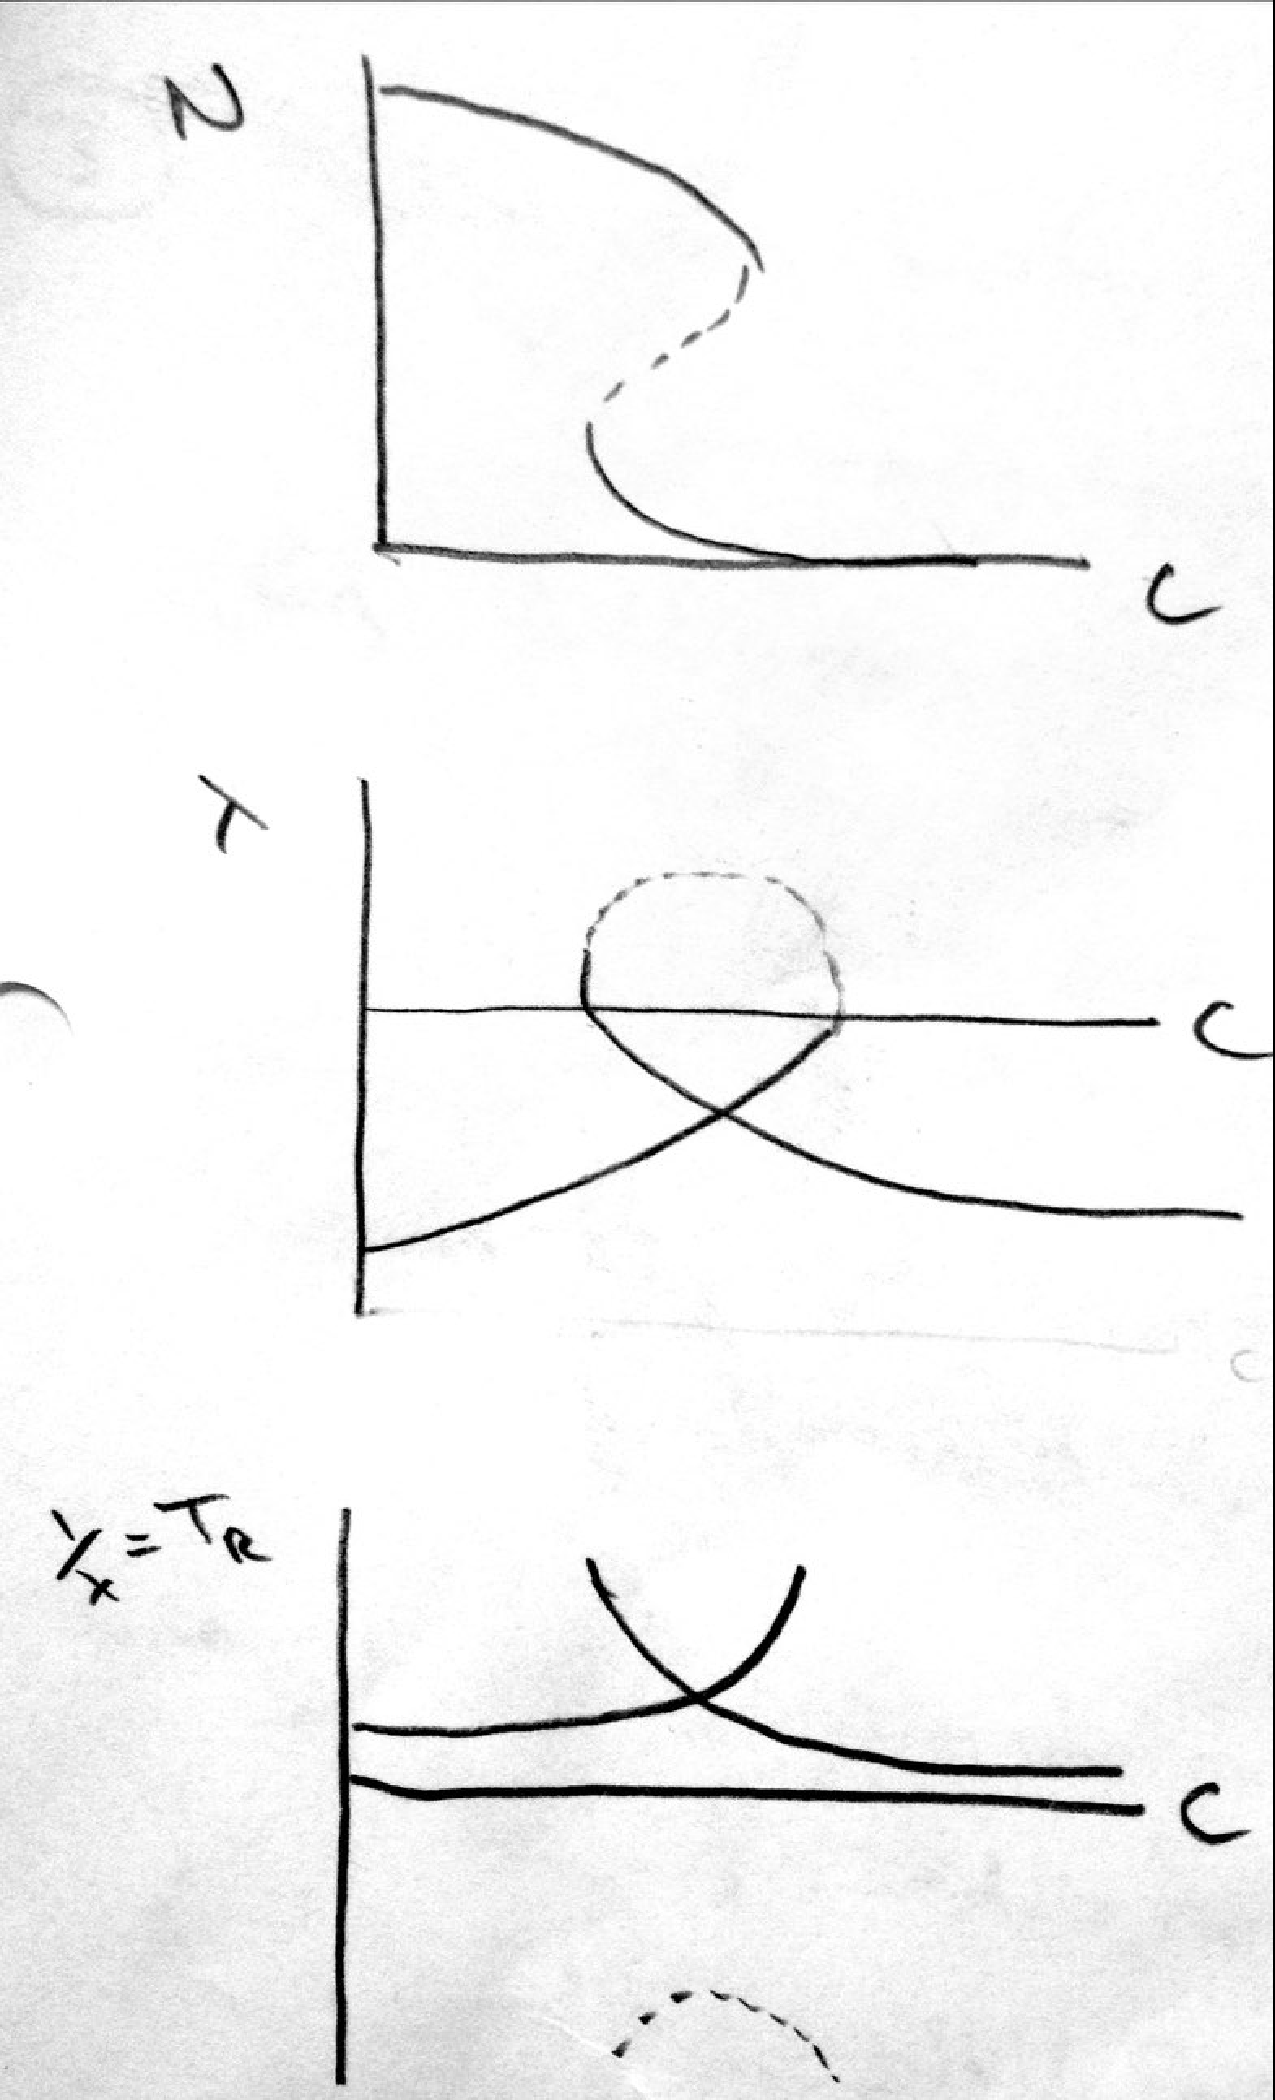
\includegraphics[width=5cm]{figs/Exploitation_CriticalSlowingDown.pdf}
 	As $\lambda \to 0, \; T_R \to \infty \quad \Rightarrow$ \emph{Critical Slowing Down}
\end{center}

Above is all about deterministic systems.  But think about real world, stochastic systems.\\
\ind i.e. \emph{Near} equilibrium,  constantly perturbed by small amounts (small pulse perturbations)\\

\begin{minipage}[t]{0.5\textwidth}
\begin{center}
	When $c < < c_2$\\
 	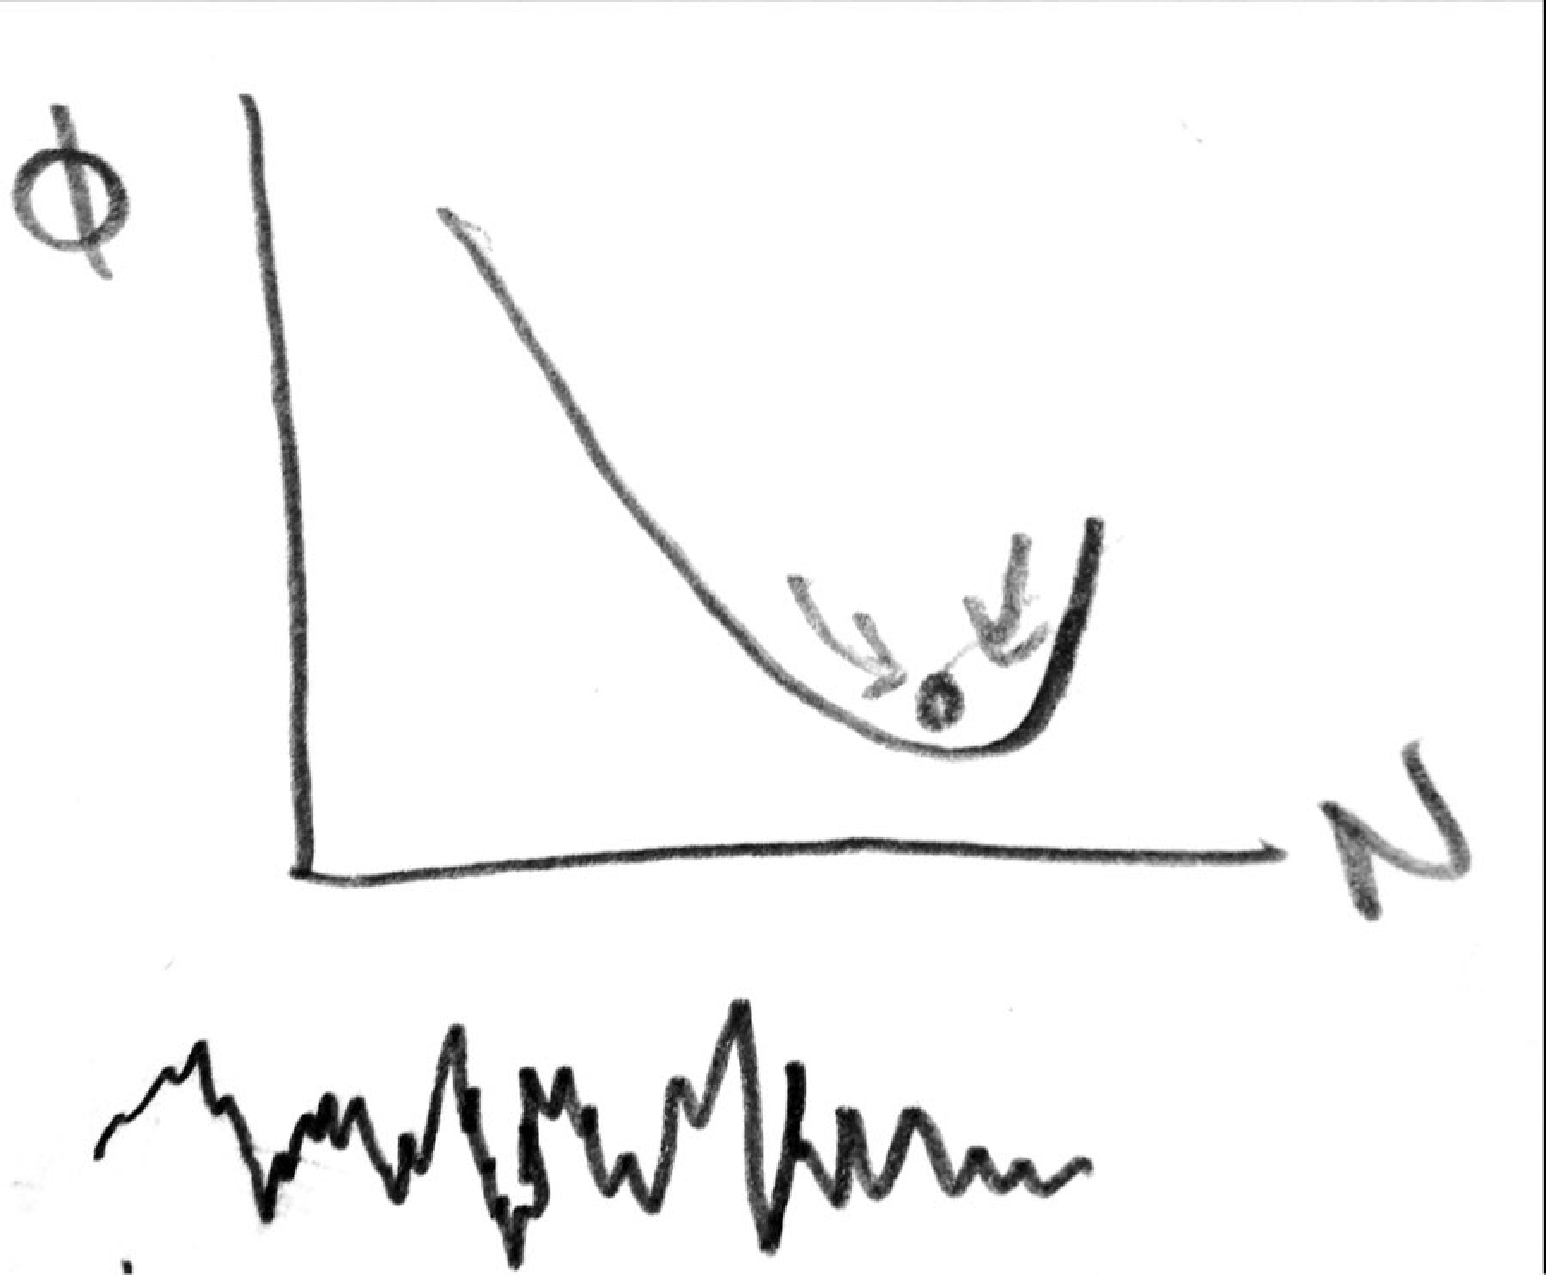
\includegraphics[width=5cm]{figs/Exploitation_Low.pdf}\\
 	Low variance\\
 	Low autocorrelation\\
 	\ind (independent and random perturbations)
\end{center}
\end{minipage}
\begin{minipage}[t]{0.5\textwidth}
\begin{center}
	As $c \to c_2$\\
 	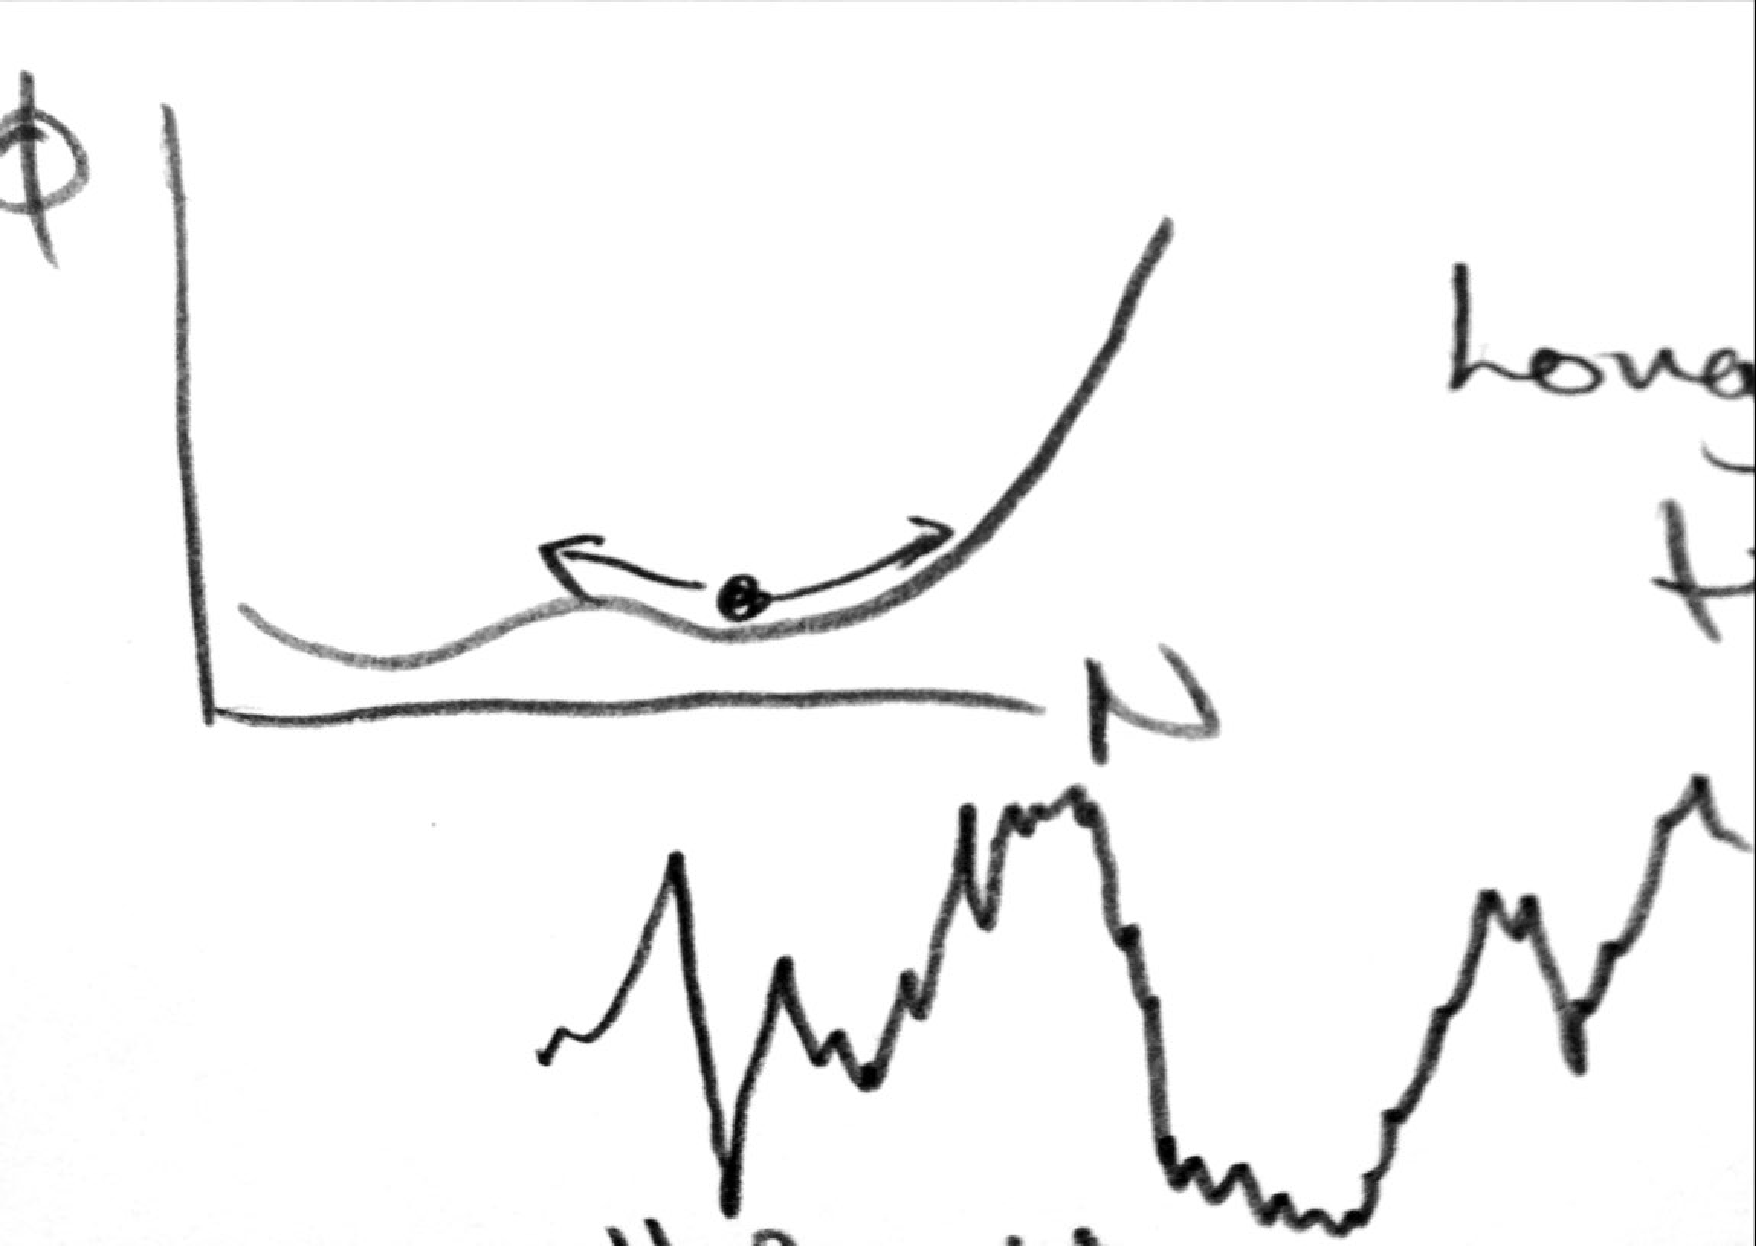
\includegraphics[width=5.5cm]{figs/Exploitation_High.pdf}\\
 	Longer return times\\
 	Higher variance\\
 	Higher autocorrelation
 	
\end{center}
\end{minipage}

\vspace{0.5cm}

Rise in variance and auto-correlation  (spatial or temporal)\\
\ind	= Early warning signal of critical bifurcation\\
	
But, note that critical slowing down occurs for bifurcation types, not just `tipping points'!\\
\ind Including Hopf bifurcations! \ind (False positives)



\rule[0.5ex]{\linewidth}{1pt}
\rule[0.5ex]{\linewidth}{1pt}



\end{document}